\documentclass[a4paper, 12pt]{article}
\usepackage[T1]{fontenc}
\usepackage[utf8]{inputenc}
\usepackage{lmodern}
\usepackage[italian]{babel}
\usepackage{graphicx}
\usepackage{amsmath}
\usepackage{hyperref}
\usepackage{listings}
\usepackage{tabularx}
\usepackage{float}
\usepackage[justification=centering]{caption}
\usepackage{subcaption}
\usepackage[
    type={CC},
    modifier={by-nc-sa},
    version={4.0},
]{doclicense}


\renewcommand{\arraystretch}{1.5}

\begin{document}

%__________FRONTESPIZIO__________

\begin{titlepage}
\begin{center}
\begin{huge}
\textbf{POLITECNICO DI TORINO}
\end{huge}

\vspace{0.5cm}

{\large Dipartimento di Ingegneria Gestionale e della Produzione}

\vspace{1cm}
\textbf{Corso di Laurea Triennale in Ingegneria Gestionale\\Classe L-8}
\vspace{1.5cm}
 
{\LARGE Tesi di Laurea Triennale\\}
 	
\vspace{1cm}

{\Large Progettazione e sviluppo di un'applicazione per la gestione di un servizio di bike sharing}

\vspace{1cm}

\includegraphics[width=0.5\textwidth]{resources/images/LogoPoliTO.pdf}
\vspace{1cm}
\end{center}
\textbf{Relatore} \hfill \textbf{Candidato}\\
Prof. Fulvio Corno \hfill Umberto Ferrari\\
\text{} \hfill Matricola 246061
\vfill

\begin{center}
{\large AA. 2019/2020}
\end{center}

\end{titlepage}

%__________INDICE__________

\tableofcontents

\newpage

\listoffigures

\listoftables

\newpage

%__________PROPOSTA__________

\section{Proposta di progetto}
	\subsection{Titolo della proposta}
	Applicazione per la gestione di un servizio di bike sharing
	
	\subsection{Descrizione del problema proposto}
	La mobilità urbana è un argomento sempre di maggior interesse, da un lato per motivi ecologici e dall'altro, attualmente, a causa dei rischi della pandemia da Covid-19. Infatti, si sta 	incentivando l'uso di mezzi di trasporto quali il bike sharing in sostituzione al normale trasporto pubblico, perciò si suppone che nei prossimi mesi si assisterà ad un aumento nel numero di utenti di questo tipo di servizi.\\\\
L'obiettivo è quello di presentare all'utente una visione d'insieme sull'utilizzo del servizio in caso di aumento dell'utenza e di fornire uno strumento adeguato a pianificare e analizzare i possibili miglioramenti da realizzare.

	\subsection{Descrizione della rilevanza gestionale del problema}
	L'applicazione intende fornire uno strumento per la gestione di un servizio di bike sharing.\\\\
Questo strumento può essere utile al gestore del servizio per metterne in luce i punti critici, per la gestione del sistema e per pianificare eventuali miglioramenti che potrebbero rivelarsi necessari a causa del probabile aumento di noleggi.

	\subsection{Descrizione dei data-set per la valutazione}
	I dati che verranno utilizzati all'interno dell'applicazione sono relativi al servizio di bike sharing della città di Londra (\href{https://www.santandercycles.co.uk/london}{Santander Cycles}):

	\begin{itemize}
	\item \textbf{Dati relativi alle stazioni di noleggio (\textit{bike points}):}\\
	I dati verranno ricavati tramite l'API fornita da TfL (\textit{Transport for London}) dal sito \url{https://api.tfl.gov.uk/} e verranno importati dal formato JSON in un database SQL tramite una funzione apposita (l'API non verrà integrata nell'applicazione, ma utilizzata una sola volta per creare il dataset).

	\item \textbf{Dati relativi ai noleggi:}\\
	I dati sui noleggi verranno estratti dal sito di \href{https://tfl.gov.uk/}{TfL} (\textit{Transport for London}) al seguente link \url{https://cycling.data.tfl.gov.uk/} dove sono disponibili suddivisi per periodo di interesse.\\
Essendo di grandi dimensioni, i dati non saranno scaricati integralmente, ma verrà inserito un unico periodo di noleggi nel database.
L'applicazione permetterà all'utente di definire un percorso per l'importazione di uno o più file di dati scaricati dal sito sopraindicato, i quali potranno essere sovrascritti o aggiunti ai dati già presenti. Anche in questo caso, i dati verranno importati dal formato CSV in un database SQL tramite una funzione apposita.
	\end{itemize}
Tutti i dati sono rilasciati con licenza \textit{\href{https://tfl.gov.uk/corporate/terms-and-conditions/transport-data-service}{Open Government Licence 2.0}} che permette il libero uso dei dati, richiedendo di riconoscere TfL come fonte delle informazioni.

	\subsection{Descrizione preliminare degli algoritmi coinvolti}
	I principali algoritmi coinvolti saranno:\\

	\begin{itemize}
	\item Un algoritmo simulativo a eventi discreti che potrà essere eseguito secondo una serie di parametri inseriti dall'utente:
		\begin{itemize}
		\item Intervallo temporale da simulare.
		\item Intervallo dei dati storici da utilizzare per effettuare la simulazione, potrà essere selezionato lo stesso periodo dell'intervallo di simulazione ma dell'anno o mese precedente, oppure si potrà selezionare manualmente l'intervallo di dati da utilizzare.
		\item Aumento dell'utenza che usufruisce del servizio, espresso in percentuale.
		\item Possibilità di attivare la ridistribuzione notturna delle bici nel sistema.
		\item Numero di bici da utilizzare durante la simulazione.
		\end{itemize}
	\item Un algoritmo che generi, sulla base dei dati "storici" inseriti e dei valori in input, i noleggi del periodo da simulare, in modo che questi ultimi non siano deterministici ma realistici rispetto ai dati inseriti.\\
Per esempio: l'aumento del traffico giornaliero inserito porterà all'inserimento di nuovi noleggi nelle ore di punta, oppure nel caso in cui siano state inserite nuove stazioni di cui non sono disponibili noleggi, l'algoritmo si occuperà di generarli tenendo conto del traffico nelle stazioni vicine.
	\end{itemize}

	\subsection{Descrizione preliminare delle funzionalità previste per l’applicazione software}
	L'applicazione prevede le seguenti funzionalità:

	\begin{itemize}
	\item Nella prima schermata verrà mostrato un riassunto dei dati relativi alle stazioni attualmente presenti nel database, in particolare sarà possibile visualizzare la mappa con la disposizione geografica delle stazioni. Inoltre, da questa schermata sarà possibile effettuare modifiche al sistema: aggiungere, sia manualmente che importando un file in formato JSON, nuove stazioni, modificarne la capienza (intesa come numero di docks) o eliminare stazioni precedentemente aggiunte.
	\item Nella seconda schermata verrà mostrato un riassunto dei dati relativi ai noleggi attualmente caricati nel database, mostrando i periodi dei gruppi di noleggi attualmente memorizzati. Inoltre sarà possibile aggiungerne di nuovi importando un file in formato CSV.
	\item Nella terza schermata sarà possibile effettuare la simulazione, eventualmente inserendo i parametri richiesti.
	Al termine della simulazione, l'utente sarà indirizzato alla quarta schermata, la quale mostrerà i risultati.
	\item Nella quarta schermata saranno mostrati i risultati relativi all'ultima simulazione eseguita, sarà possibile visualizzare una mappa con indicate le stazioni codificate secondo una scala di colore rispetto al problema più rilevante che vi si è verificato. In particolare, tali problemi possono essere:
		\begin{itemize}
		\item Stazioni vuote, quindi utenti che non sono riusciti a noleggiare una bicicletta.
		\item Stazioni piene in cui gli utenti non sono riusciti a consegnare la bicicletta, dovendosi quindi recare in un'altra stazione per terminare il noleggio.
		\item Stazioni ad alto traffico, per cui sarebbe utile un miglioramento.
		\end{itemize}
	Inoltre, da questa schermata sarà possibile visualizzare dei grafici che riassumono i risultati della simulazione.
	\end{itemize}

\newpage

%__________DESCRIZIONE PROBLEMA AFFRONTATO__________

\section{Descrizione dettagliata dal problema}

	\subsection{Servizi di bike sharing}

	I servizi di bike sharing sono uno strumento di mobilità alternativa e sostenibile che negli ultimi anni ha visto una sempre maggior diffusione, anche sul territorio italiano.\\
	Questi servizi mettono a disposizione un parco bici da poter essere noleggiato in autonomia dagli utenti. \\
	La necessità di queste tipologie di servizio e il loro miglioramento è dovuto ai sempre maggiori problemi di mobilità presenti ormai nella maggior parte delle città del mondo, anche in ottica ambientale l'ampliamento di questi servizi porterebbe giovamenti rilevanti. \\Inoltre, a seguito della pandemia da Covid-19 si sta incentivando l'uso di mezzi di trasporto alternativi, quali bike sharing e car sharing, in sostituzione al normale trasporto pubblico a causa del rischio sanitario legato all'utilizzo di bus, metropolitane e tram.\\\\
	I servizi di bike sharing si dividono in due categorie fondamentali: 
	\begin{itemize}
		\item \textbf{Station-based}: il servizio si basa sul posizionamento sul territorio di un certo numero di postazioni (stazioni appunto) in cui noleggiare e riconsegnare i mezzi.
		\item \textbf{Free-floating}: si tratta di servizi a flusso libero, in linea generale permettono di noleggiare e riconsegnare la bici in qualsiasi punto dell'area di copertura del servizio.
	\end{itemize}
La prima tipologia è diffusa ormai da molti anni, mentre la seconda si è sviluppata solo di recente a causa delle maggiori difficoltà tecnologiche e di gestione ad essa connesse.\\
La città di Torino ne è un esempio: è stato inaugurato il servizio di bike sharing \href{http://www.tobike.it/default.aspx}{[TO]Bike} a postazioni fisse nel 2010, ma soltanto nel 2017 è arrivato il primo servizio free-floating \href{https://mobike.com/global/}{Mobike}.\\\\
Nello sviluppo di questa applicazione si sono presi in considerazione i servizi della tipologia station-based.

\newpage

	\subsection{Obiettivi}

	L'obiettivo di questa applicazione è duplice. \\
Da un lato, permettere al gestore di un servizio di bike sharing di avere una visione d'insieme sullo stato del servizio e metterne in luce i punti critici. \\ 
Dall'altro, l'applicazione potrà essere utilizzata per analizzare le conseguenze dovute a modifiche al sistema, testando, in particolare i possibili benefici che si potrebbero avere a seguito dell'ampliamento del sistema con l'installazione di nuove stazioni o con l'ampliamento del parco mezzi messo a disposizione degli utenti.\\\\
Nello specifico, questi obiettivi sono stati realizzati per mezzo di una simulazione dell'utilizzo del sistema da parte degli utenti. Il gestore del servizio potrà agire sui parametri di simulazione o effettuare modifiche al sistema per verificare l'uso del servizio sotto determinate condizioni. \\ Per esempio, sarà possibile verificare le zone critiche del sistema nel caso di un consistente aumento dell'utenza che usufruisce del servizio, oppure i benefici che si potrebbero avere in caso di installazione di una nuova stazione in una particolare area.\\\\
Infine, attivando la funzionalità relativa, sarà possibile visualizzare i benefici legati alla realizzazione di una strategia di ridistribuzione dei mezzi all'interno del sistema durante le ore notturne.\\\\\\
L'applicazione fornirà, oltre che una serie di parametri numerici e grafici, anche una mappa interattiva in cui sarà possibile visualizzare tutte le stazioni del sistema suddivise a seconda del problema più rilevante verificatosi. In particolare, si è deciso di suddividere le stazioni in quattro categorie:
	\begin{itemize}
		\item \textbf{Nessun problema rilevante}: una stazione viene inserita in questa categoria se tutti gli indicatori che identificano le tre categorie sottostanti sono al di sotto della media relativa a tutte le stazioni.
		\item \textbf{Stazioni spesso vuote}: stazioni in cui vi è stato un numero di utenti che ha tentato di effettuare un noleggio trovando però la stazione vuota, molto sopra la media di questo stesso numero, calcolata rispetto a tutte le stazioni. E' stato ritenuto il problema più grave che si possa verificare, in quanto oltre che a causare un disservizio per gli utenti, genera anche una perdita economica per il gestore.
		\item \textbf{Stazioni spesso piene}: stazioni in cui vi è stato un numero di utenti che ha tentato di riconsegnare la bici noleggiata trovando però la stazione piena, molto sopra la media di questo stesso numero, calcolata rispetto a tutte le stazioni. Anche in questo caso, si tratta di un problema rilevante, ma che non causa una perdita economica diretta al gestore. In particolare, questa criticità può essere ridotta, almeno in parte, avviando una strategia di ridistribuzione del parco mezzi nel sistema, come dimostrato utilizzando la funzionalità apposita che simula una delle possibili strategie.
		\item \textbf{Stazioni ad alto traffico}: stazioni con un elevato numero di utenti durante il periodo in esame, nelle quali si è verificato almeno un problema in maniera consistente, ma non sufficiente per ricadere in una delle categorie di cui sopra.
	\end{itemize}

	\subsection{Criticità}
	\label{crit}

	Le principali criticità sono legate ad alcuni parametri reali di cui non è stato possibile tenere conto.\\\\
	In primo luogo, a causa della mancanza di informazioni non è stato possibile tenere conto di eventuali danneggiamenti e conseguente riparazione dei mezzi.\\\\
	Inoltre, molti servizi offrono ai propri utenti minuti di noleggio gratuiti in caso in cui incorrano in una serie di problemi, per esempio una stazione vuota; ovviamente questo fatto aumenta la tendenza degli utenti a recarsi in una nuova stazione per effettuare il noleggio. Per ovvi motivi non è stato possibile tenere conto di questa variabile, si è però tentato di sopperire al problema chiedendo all'utente, in fase di avvio della simulazione, di inserire un parametro che indichi la tendenza degli utenti del servizio a cercare una nuova stazione nel caso in cui incorrano in problemi.\\\\
	Infine, per quanto riguarda la funzione di ridistribuzione notturna, la strategia implementata è solo una delle possibili e non è di certo universalmente utile. In altre parole, non per tutti i servizi una strategia di questo tipo potrebbe portare reali benefici tali da giustificarne la messa in pratica, infatti ogni gestore, soprattutto sulla base della conformazione dell'area del servizio, elabara una propria strategia di ridistribuzione. Quella che è stata presa in considerazione è la più generale e indipendente dalla conformazione dell'area di copertura. Si è voluto inserire questa funzionalità solo per dare un'idea, per quanto generale, della possibile utilità di azioni di questo tipo.

\newpage

%__________DATASET__________

\section{Dataset}
I dati utilizzati dall'applicazione sono di due tipi principali:
\begin{itemize}
	\item Dati relativi alle stazioni di noleggio (\textit{stations})
	\item Dati relativi ai noleggi (\textit{rentals})
	\item In aggiunta, vengono utilizzate le informazioni relative alle biciclette presenti nel sistema, in particolare la sola informazione sull'ID del mezzo, la presenza di queste informazioni è però totalmente facoltativa, l'applicazione è strutturata per funzionare anche nel caso in cui la tabella \textit{bike} sia vuota, provvedendo a generare gli ID dei mezzi a seconda del numero di bici da utilizzare per la simulazione inserito dall'utente.
\end{itemize}
Il software è stato realizzato per poter funzionare con i dati relativi a qualsiasi servizio, semplicemente importando i dati necessari tramite le funzionalità di caricamento file presenti.\\\\
A scopo di esempio e per permettere di testare le funzionalità dell'applicazione è stato scelto di utilizzare i dati relativi al servizio di bike sharing \href{https://www.santandercycles.co.uk/london}{Santander Cycles} della città di Londra, dati messi a disposizione dall'ente \href{https://tfl.gov.uk/}{Trasport for London} (\textit{TfL}) e rilasciati con licenza \textit{\href{https://tfl.gov.uk/corporate/terms-and-conditions/transport-data-service}{Open Government Licence 2.0}}.
\begin{itemize}
	\item I dati relativi alle stazioni sono stati ricavati tramite l'\href{https://api.tfl.gov.uk/}{API} fornita da TfL, è stato estratto il file testuale in formato JSON contenente le informazioni necessarie per poi essere importato nel database SQL.
	\item I dati relativi ai noleggi sono stati estratti al seguente indirizzo  \url{https://cycling.data.tfl.gov.uk/} dove sono disponibili in formato CSV, per poi essere importati nel database SQL. Al link indicato è possibile, inoltre, scaricare ulteriori dati per poter ampliare il dataset proposto.
\end{itemize}

\newpage

\begin{figure}
\caption{Diagramma ER}
\label{diagramer}
\hfill 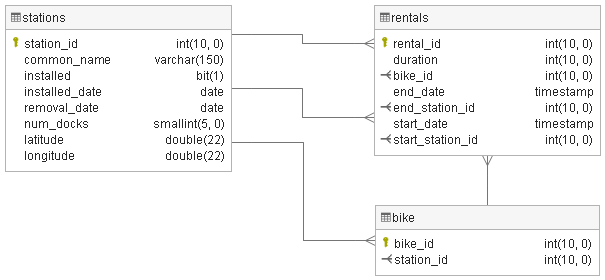
\includegraphics[width=\textwidth]{resources/images/DiagrammaER.png} \hspace*{\fill}
\end{figure}	

	\subsection{Descrizione delle tabelle}

	\subsubsection{Tabella stations}

	La tabella \textit{stations} contiene le informazioni relative alle stazioni presenti nel sistema:
	
	\begin{itemize}
		\item station\_id: ID della stazione.
		\item common\_name: nome della stazione.
		\item installed: parametro di tipo binario, serve a identificare le stazioni ancora installate nel sistema rispetto a quelle ormai rimosse, l'applicazione in fase di simulazione considererà le sole stazioni che presentano questo parametro a 1.
		\item installed\_date e removal\_date: rispettivamente data di installazione e di rimozione della stazione, nel caso in cui la stazione sia installata il campo removal\_date assume valore \textit{null}.
		\item num\_docks: capienza della stazione intesa come numero di colonnine presenti.
		\item latitude e longitude: latitudine e longitudine del punto in cui si trova la stazione.
	\end{itemize}

	\subsubsection{Tabella rentals}

	La tabella \textit{rentals} contiene le informazioni relative ai noleggi che sono stati effettuati dagli utenti del sistema, sulla base di questi dati l'applicazione genererà gli eventi di noleggio per effettuare la simulazione.

	\begin{itemize}
		\item rental\_id: ID del noleggio.
		\item duration: durata del noleggio, espressa in secondi.
		\item bike\_id: ID della bici utilizzata nel noleggio.
		\item start\_date e end\_date: campi di tipo timestamp che rappresentano data e ora rispettivamente di inizio e fine noleggio.
		\item start\_station\_id e end\_station\_id: ID della stazione in cui avviene rispettivamente il prelevamento e la riconsegna della bici.
	\end{itemize}

	\subsection{Formato dei file da importare}

	Tutti i dati possono essere importati tramite file, di seguito si descrive brevemente il formato di questi file per l'utilizzo dell'applicazione con dati relativi ad altri servizi.\\\\
Per poter importare dati relativi alle stazioni è necessario realizzare un file testuale in formato JSON con la seguente struttura.\\
	
	\lstinputlisting{resources/FileStazioni.txt}

	\text{}\\
Per poter importare dati relativi ai noleggi è necessario realizzare un file in formato CSV utilizzando la virgola come separatore.\\ L'ordine dei parametri per ogni riga deve essere il seguente.\\

	\begin{lstlisting}[breaklines=true]
Rental Id,Duration,Bike Id,End Date,EndStation Id,EndStation Name,Start Date,StartStation Id,StartStation Name
100,60,1,01/01/2020 12:00,5,"Nome stazione arrivo",01/01/2020 13:00,7,"Nome stazione partenza"
	\end{lstlisting}

\newpage

%__________STRUTTURE DATI E ALGORITMI__________

\section{Strutture dati e algoritmi utilizzati}

	\subsection{Struttura del progetto}
	
	L'applicazione è stata sviluppata in linguaggio Java, seguendo i pattern MVC (\textit{Model-View-Controller}) e DAO (\textit{Database Access Object}).\\\\
	Il progetto dell'applicazione è disponibile nel repository \href{https://github.com/}{GitHub} al seguente link: \url{https://github.com/TdP-prove-finali/FerrariUmberto}.\\\\
	Il progetto si compone di 5 package, ognuno dedicato allo svolgimento di determinate funzionalità.\\

	\begin{table}
	\begin{center}
	\caption{Schema dei package}
	 \begin{tabular}{| c | c |  c |} 
	 \hline
	 \textbf{Nome del package} & \textbf{Numero di classi} & \textbf{Descrizione} \\ [0.5ex] 
	\hline
	 \hline
	 CompassBike & 2 & Avvio dell'applicazione \\
	 \hline
	 controller & 7 & Controller interfaccia grafica \\  
	 \hline
	 model & 11 & Algoritmi \\
	 \hline
	 DAO & 4 & Collegamento al database \\
	 \hline
	 dataImport & 6 & Importazione dei dati \\
	 \hline
	\end{tabular}
	\end{center}
	\end{table}

	\begin{itemize}
		\item \textbf{CompassBike}: contiene le classi per l'avvio dell'applicazione.
		\item \textbf{controller}:  dedicato al controllo dell'interfaccia grafica, è presente una classe \textit{controller} per ogni schermata dell'interfaccia, la classe \textit{ChangePage} permette il cambio di interfaccia e gestisce la schermata di caricamento; infine, la classe \textit{MapsGenerator} si occupa di realizzare le mappe interattive.
		\item \textbf{model}:  package principale dell'applicazione, contiene la parte algoritmica e le classi necessarie alla memorizzazione dei dati.
		\item \textbf{DAO}: dedicato alle interazioni dell'applicazione con il database: connessione al database, lettura e modifica dei dati memorizzati.
		\item \textbf{dataImport}: gestisce le funzionalità di importazione dati.
	\end{itemize}

\newpage

	\subsection{Software e librerie}

	L'applicazione è stata sviluppata tramite l'IDE \href{https://www.eclipse.org/}{Eclipse}. Per la realizzazione di parte dell'interfaccia grafica è stato utilizzato il software \href{https://gluonhq.com/products/scene-builder/}{SceneBuilder}.\\\\
	Il DBMS utilizzato è \href{https://mariadb.org/}{MariaDB} con interfaccia grafica \href{https://www.heidisql.com/}{HeidiSQL}.\\
	A causa dell'uso di alcuni comandi SQL che presentano notazioni differenti a seconda del DBMS utilizzato, non si assicura il funzionamento dell'applicazione con DBMS diversi da MariaDB.\\\\\\
Per lo sviluppo dell'applicazione sono state utilizzate le seguenti librerie, importate nel progetto, con la sola eccezione dell'ultima sotto riporata, tramite l'uso di \textit{Maven}, inserendo la relativa \textit{dependency} all'interno del file \textit{pom.xml}.

	\begin{itemize}
		\item \href{https://github.com/stleary/JSON-java}{JSON-Java}: utilizzata per facilitare l'importazione di file testuali in formato JSON.
		\item \href{https://jgrapht.org/}{JGraphT}: utilizzata per la realizzazione dei grafi.
		\item \href{http://www.jfoenix.com/}{JFoenix}: libreria di oggetti JavaFX material design.
		\item \href{https://github.com/Jerady/fontawesomefx-glyphsbrowser}{FontAwesomeFX}: utilizzata per alcune aggiunte all'interfaccia dell'applicazione.
		\item \href{https://docs.mapbox.com/mapbox-gl-js/api/}{MapBox GL}: si tratta di una libreria in linguaggio \textit{JavaScript}, è stata utilizzata per la realizzazione delle mappe interattive.
	\end{itemize}

	

\newpage

	\subsection{Algoritmi}

	L'applicazione si compone di due algoritmi principali.

	\subsubsection{Algoritmo di generazione eventi}

		Lo scopo di questo algoritmo, contenuto nella classe \textit{EventsGenerator}, è quello di generare gli eventi su cui effettuare la simulazione. In particolare, genera gli eventi secondo i parametri inseriti dall'utente e i dati relativi ai noleggi contenuti nel database.\\\\
		Questo algoritmo utilizza la maggior parte delle funzioni contenute nelle classi del package DAO, per ottenere informazioni aggregate dei dati memorizzate nel database. Sulla base dei dati ottenuti vengono create una serie di strutture dati necessarie all'esecuzione dell'algoritmo, in particolare:

	\begin{itemize}
		\item Un grafo diretto e pesato, i nodi rappresentano le stazioni e gli archi, rappresentati dalla classe \textit{RouteEdge}, contengono le informazioni relativi ai tempi minimi e massimi di percorrenza del tragitto tra le due stazioni connesse dall'arco.
		\item Una serie di mappe che contengono varie informazioni, ad esempio, la probabilità che un utente del servizio si rechi in una certa stazione per effettuare un noleggio o la distribuzione del numero di noleggi effettuati nei diversi giorni e nei diversi istanti di tempo.\\
	\end{itemize}
Una seconda parte dell'algoritmo permette di generare i dati sopra descritti anche per le stazioni inserite manualmente dall'utente o comunque per quelle stazioni per cui non sono disponibili dati memorizzati nel database. La generazione di questi parametri si basa sull'analisi dei valori associati alle 5 stazioni più vicine a quella in esame.
In particolare, l'inserimento di una stazione in una certa area porterà a un aumento di traffico nella zona, ma anche a un reindirizzamento di una parte delle operazioni effettuate nelle stazioni più vicine nella nuova stazione.\\\\
L'algoritmo restituisce una lista di \textit{Event} di tipo \textit{Noleggio}, che rappresentano quindi la volontà di un utente di iniziare un noleggio in una certa stazione in un certo istante di tempo. Questi dati sono scelti casualmente sulla base dei parametri sopra descritti.


		\subsubsection{Algoritmo di simulazione}

		La parte principale dell'applicazione è composta dall'algoritmo di simulazione a eventi discreti, contenuto nella classe \textit{Simulator}, che riceve in input i parametri inseriti dall'utente e la lista di eventi generati e si occupa di simulare tutte le operazioni effettuate nel sistema.\\\\
		La classe \textit{Simulator}, tramite una funzione apposita, si occupa anche di inizializzare le bici all'interno del sistema. La disposizione avviene in maniera uniforme, tentando di portare tutte le stazioni allo stesso tasso di riempimento, dando però priorità a stazioni a maggior capienza.\\\\
Nella tabella \ref{eventtype} è riportata una descrizione delle tipologie di evento utilizzate nell'algoritmo di simulazione.\\\\
La figura \ref{flowchart} mostra tramite un flowchart le operazioni gestite dall'algoritmo di simulazione.

		\begin{table}
		\caption{Schema eventi simulazione}
		\label{eventtype}
		\begin{tabularx}{\textwidth}{| l | X |}
		 \hline
		 \textbf{Tipo} & \textbf{Descrizione} \\ [0.5ex] 
		 \hline
		 \hline
		Noleggio & Rappresenta la volontà di un utente ad iniziare un noleggio \\ 
		 \hline
		Prelievo & Rappresenta l'inizio effettivo del noleggio con il prelevamento della bici da parte dell'utente \\
		 \hline
		Rilascio &  Rappresenta il termine del noleggio con la riconsegna della bici \\
		 \hline
		Stazione piena &  Generato da un evento di \textit{Rilascio} nel caso in cui la stazione di riconsegna scelta non abbia colonnine libere \\
		 \hline
		Stazione vuota &  Generato da un evento di tipo \textit{Noleggio} nel caso in cui non siano disponibili delle bici nella stazione scelta per il prelevamento \\
		 \hline
		\end{tabularx}
		\end{table}

		\begin{figure}
		\caption{Flowchart simulazione}
		\label{flowchart}
		\hfill 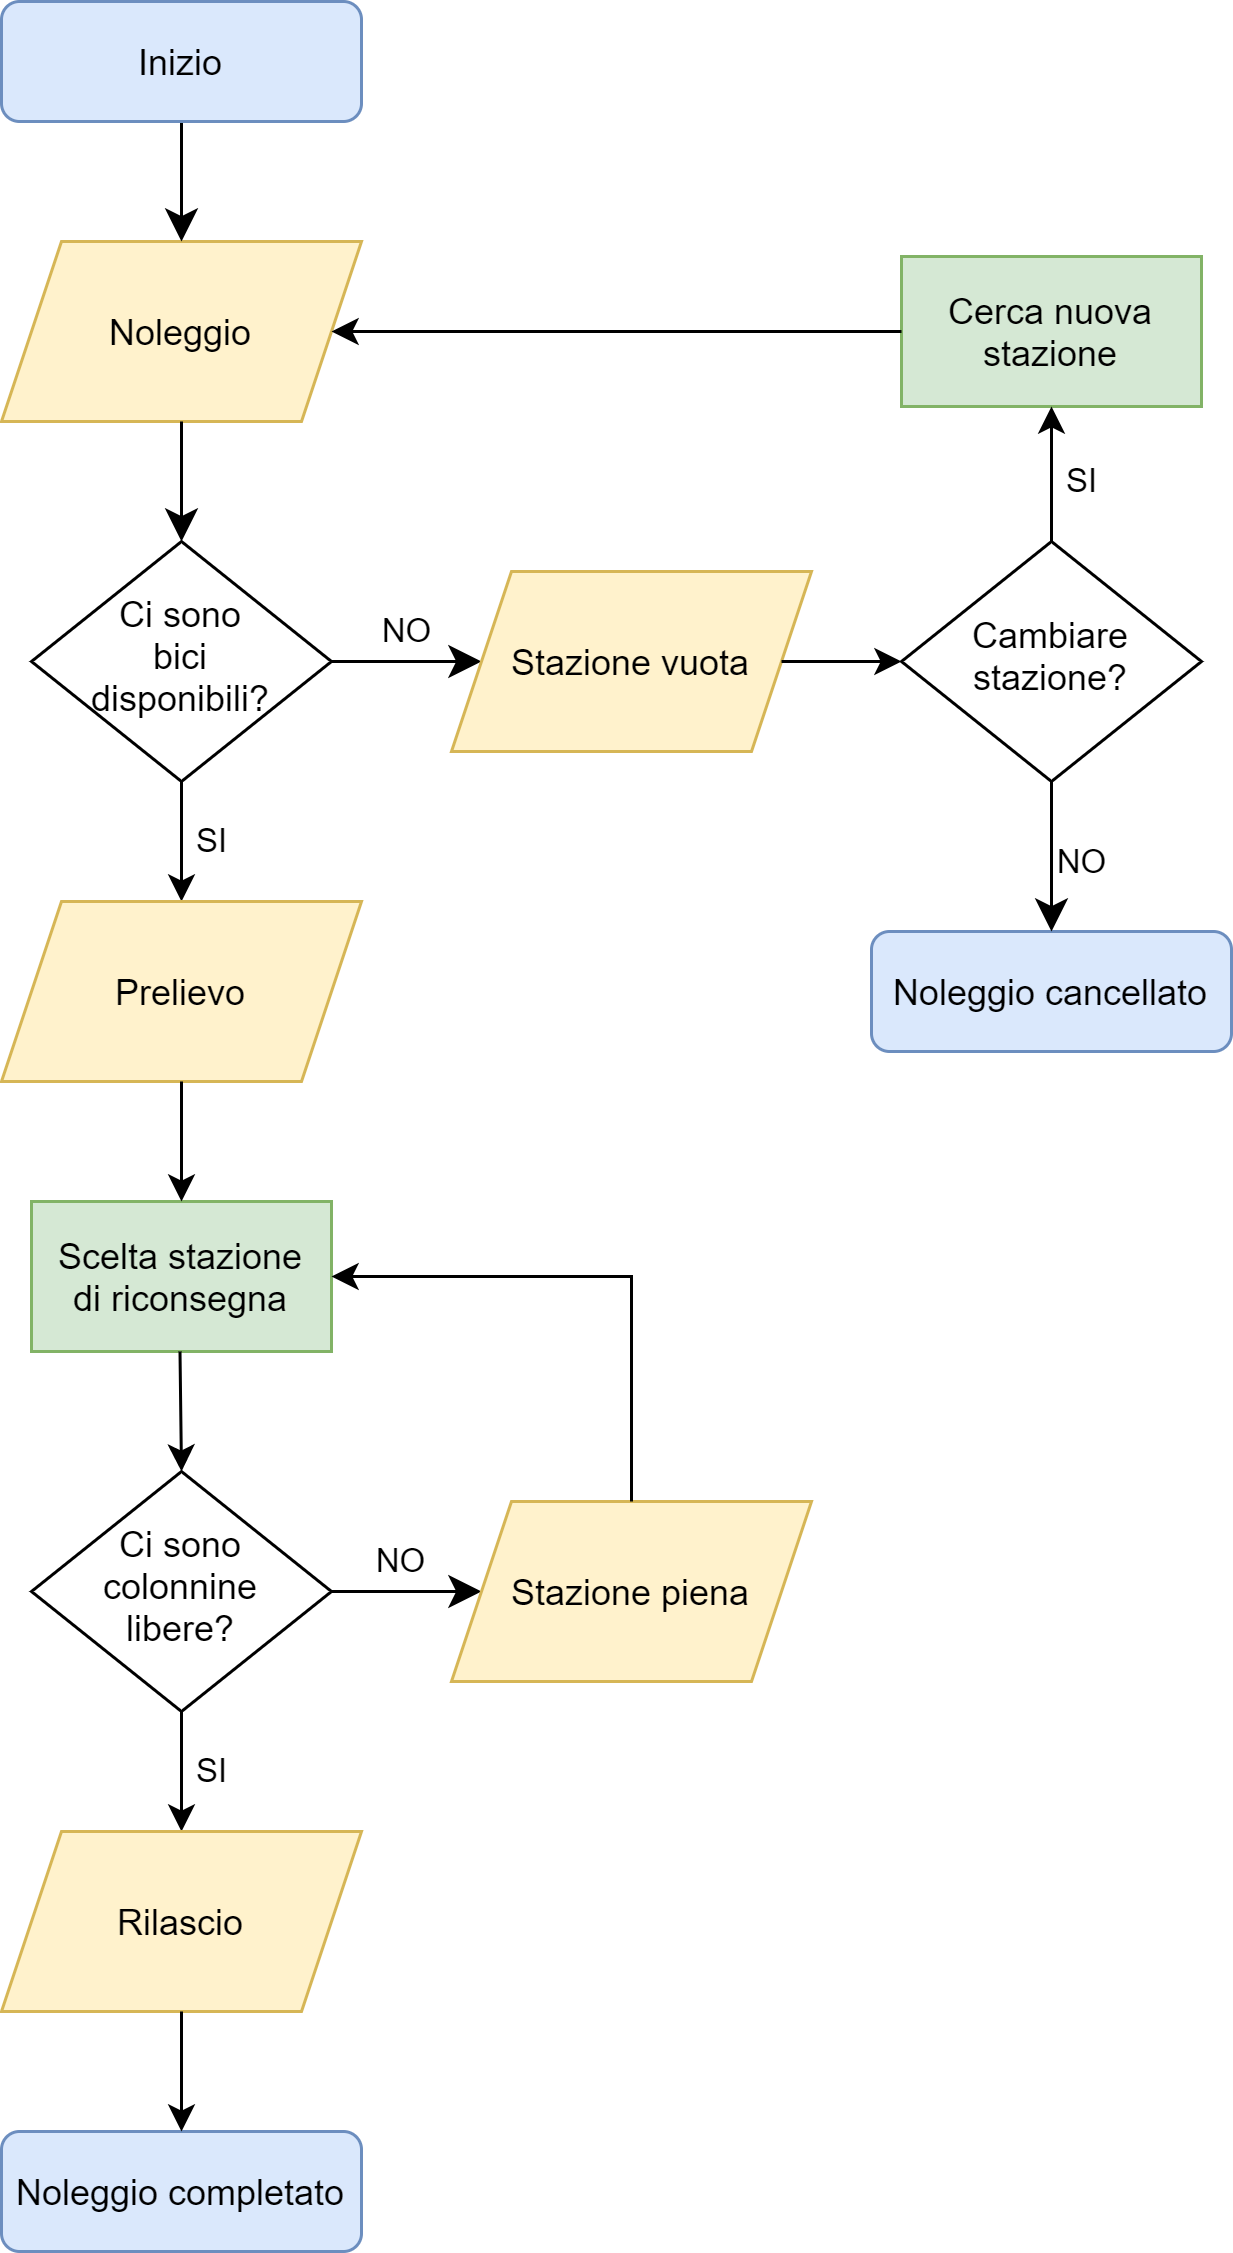
\includegraphics[height=\textheight]{resources/images/FlowChart.png} \hspace*{\fill}
		\end{figure}	

\newpage

%__________DIAGRAMMA CLASSI__________

\section{Diagramma delle classi principali}
	\begin{figure}[H]
	\caption{Diagramma UML package DAO}
	\label{umldao}
	\hfill 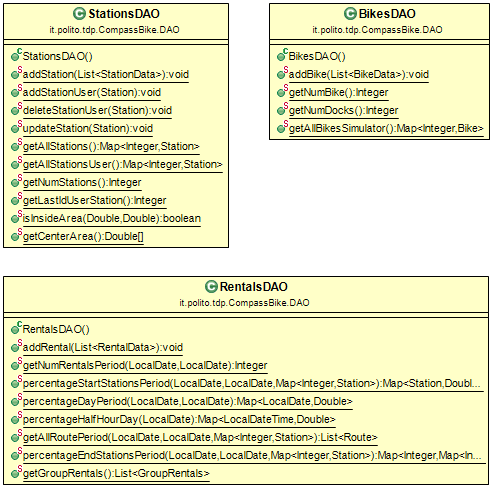
\includegraphics[height=0.45\textheight]{resources/images/UML/UMLDAO.png} \hspace*{\fill}
	\caption{Diagramma UML package dataImport}
	\label{umldata}
	\hfill 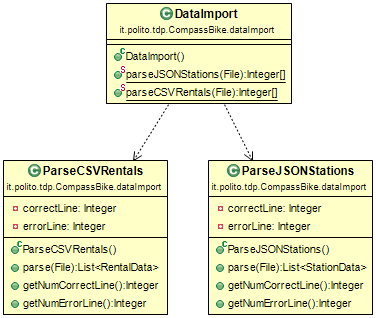
\includegraphics[height=0.35\textheight]{resources/images/UML/UMLDataImport.png} \hspace*{\fill}
	\end{figure}	
	\begin{figure}[H]
	\caption{Diagramma UML package model}
	\label{umlmodel}
	\hfill 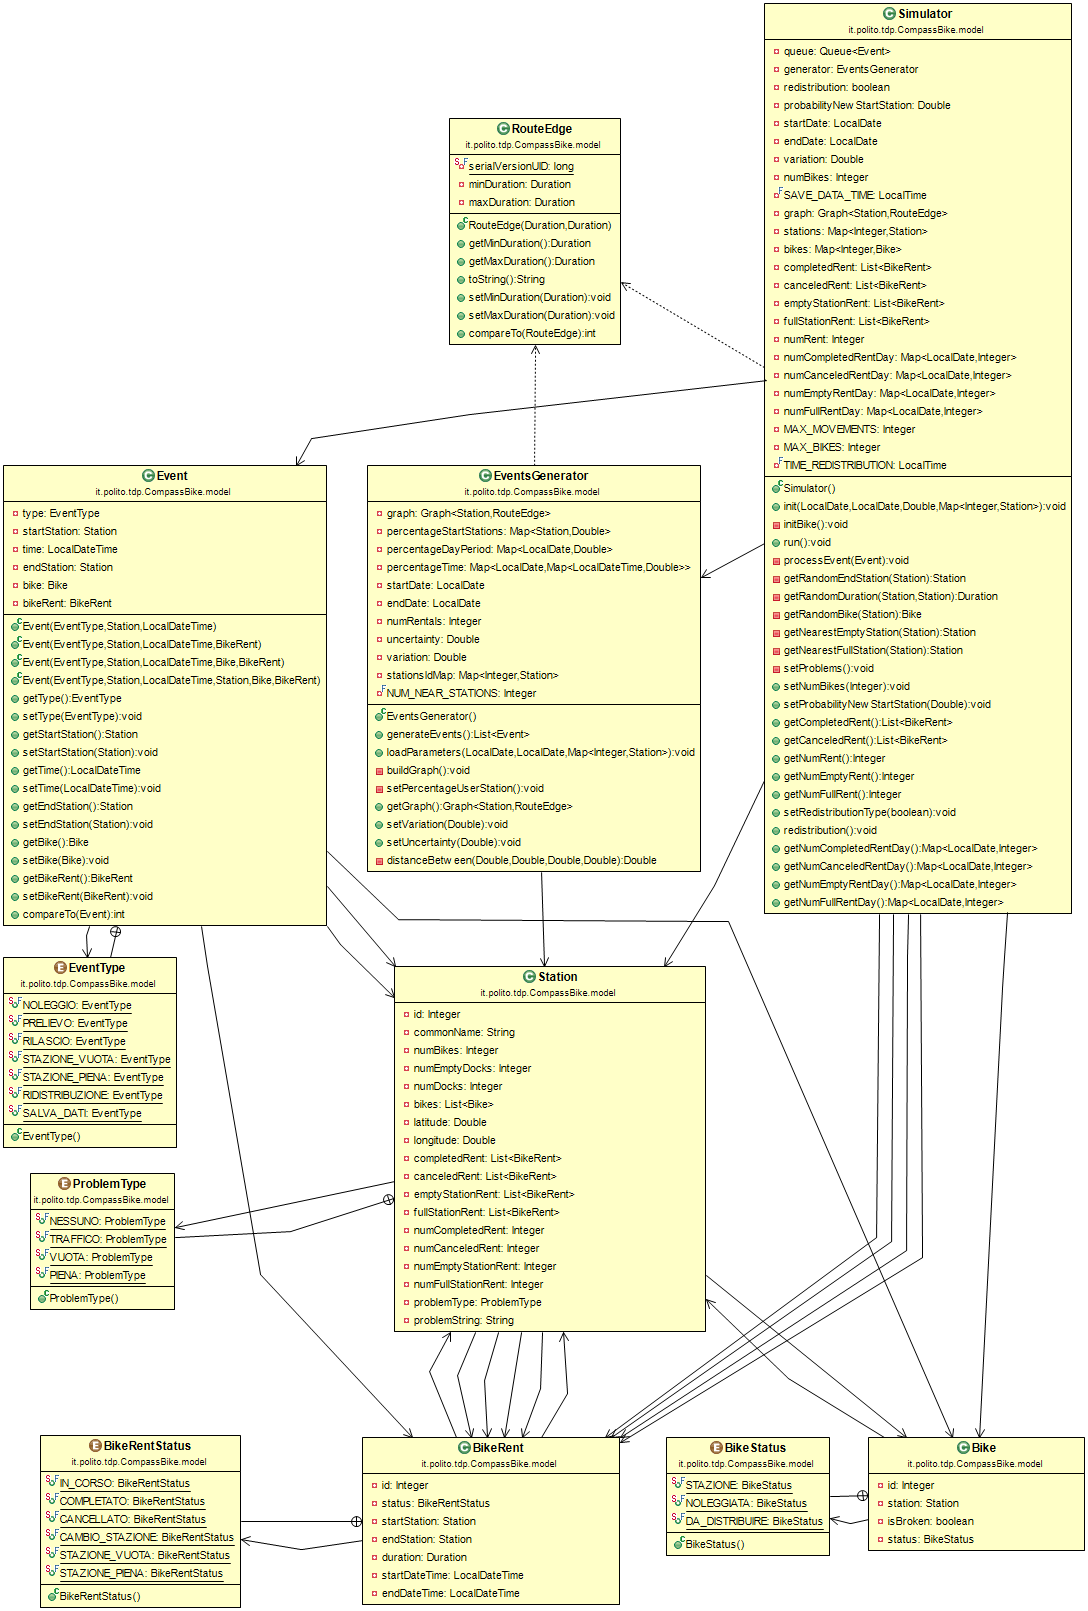
\includegraphics[height=0.95\textheight]{resources/images/UML/UMLmodel.png} \hspace*{\fill}
	\end{figure}	

\newpage

%__________INTERFACCIA__________

\section{Interfaccia dell'applicazione}

L'applicazione si compone di 4 schermate, inoltre, tramite un apposito pulsante è possibile aprire il browser per visualizzare le mappe interattive, oppure aprire una nuova finestra che mostra i risultati della simulazione sotto forma di grafici.\\
E' stato realizzato un video dimostrativo sull'uso dell'applicazione, disponibile al link: \url{https://youtu.be/wRPsn2E0DYg}.

	\begin{figure}[H]
	\caption{Schermata inserimento dati stazioni}
	\label{stationsdata}
	\hfill 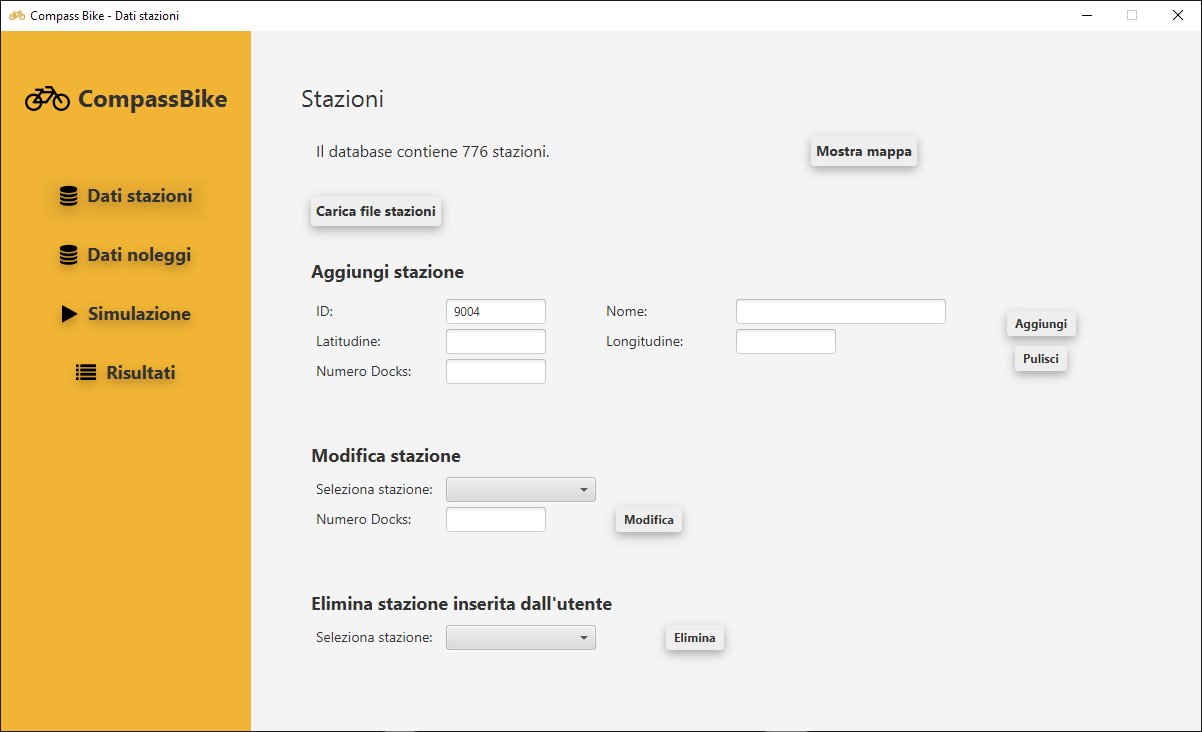
\includegraphics[height=0.34\textheight]{resources/images/screenshot/StationsData.png} \hspace*{\fill}

	\caption{Schermata inserimento dati noleggi}
	\label{rentalsdata}
	\hfill 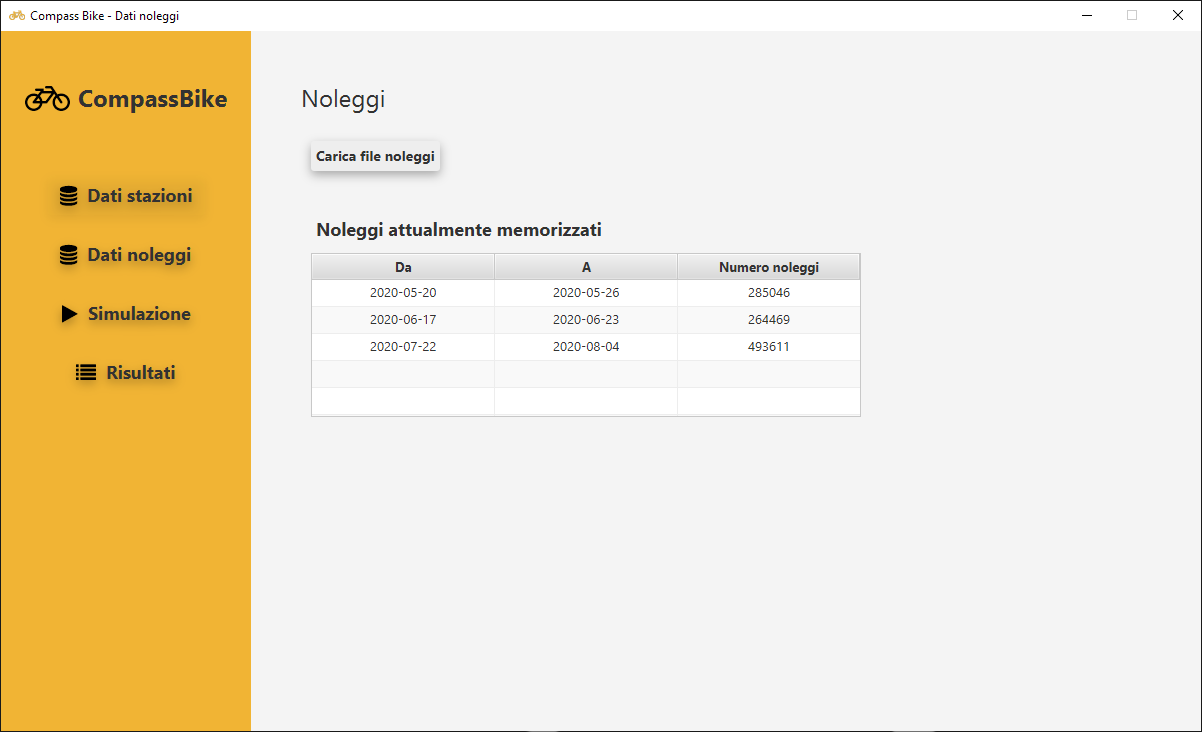
\includegraphics[height=0.34\textheight]{resources/images/screenshot/RentalsData.png} \hspace*{\fill}
	\end{figure}	

	\begin{figure}[H]
	\caption{Schermata avvio simulazione}
	\label{simulation}
	\hfill 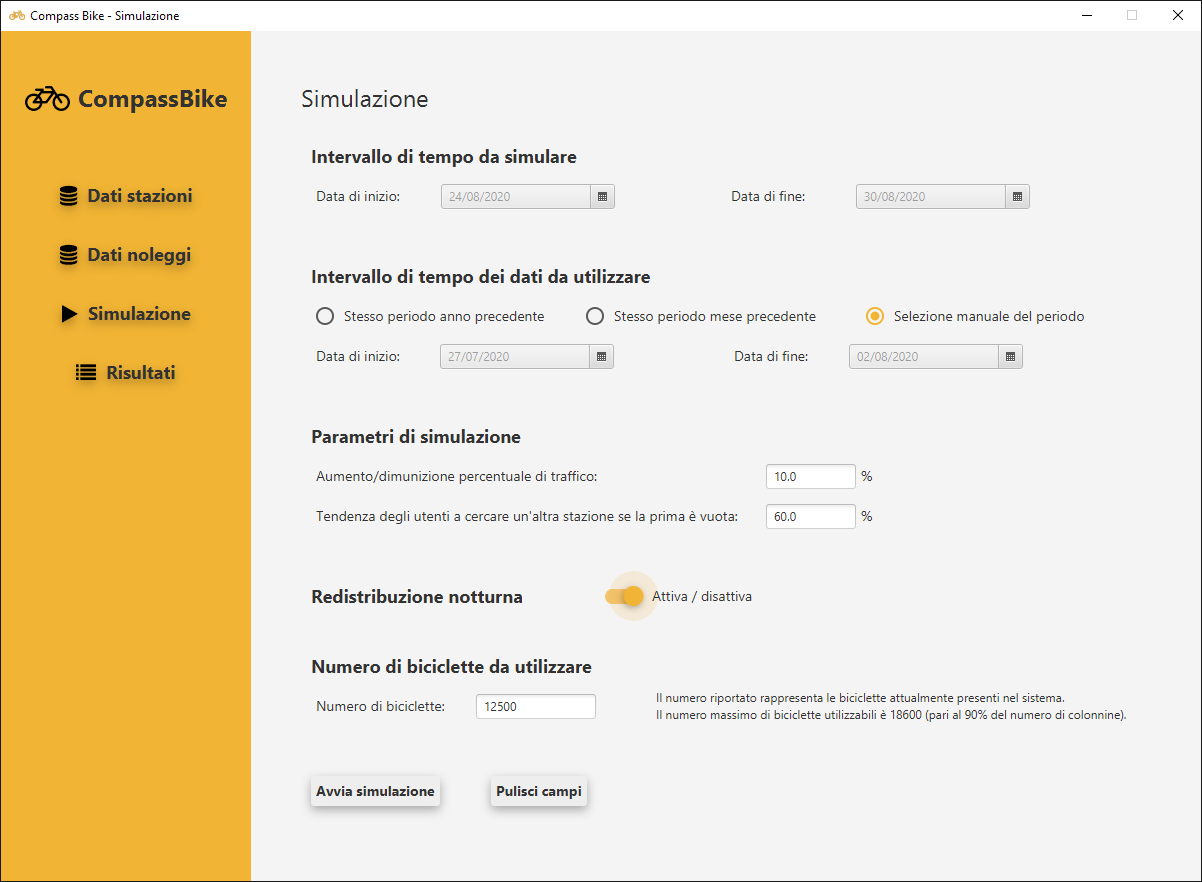
\includegraphics[height=0.47\textheight]{resources/images/screenshot/Simulation.png} \hspace*{\fill}

	\caption{Schermata risultati}
	\label{result}
	\hfill 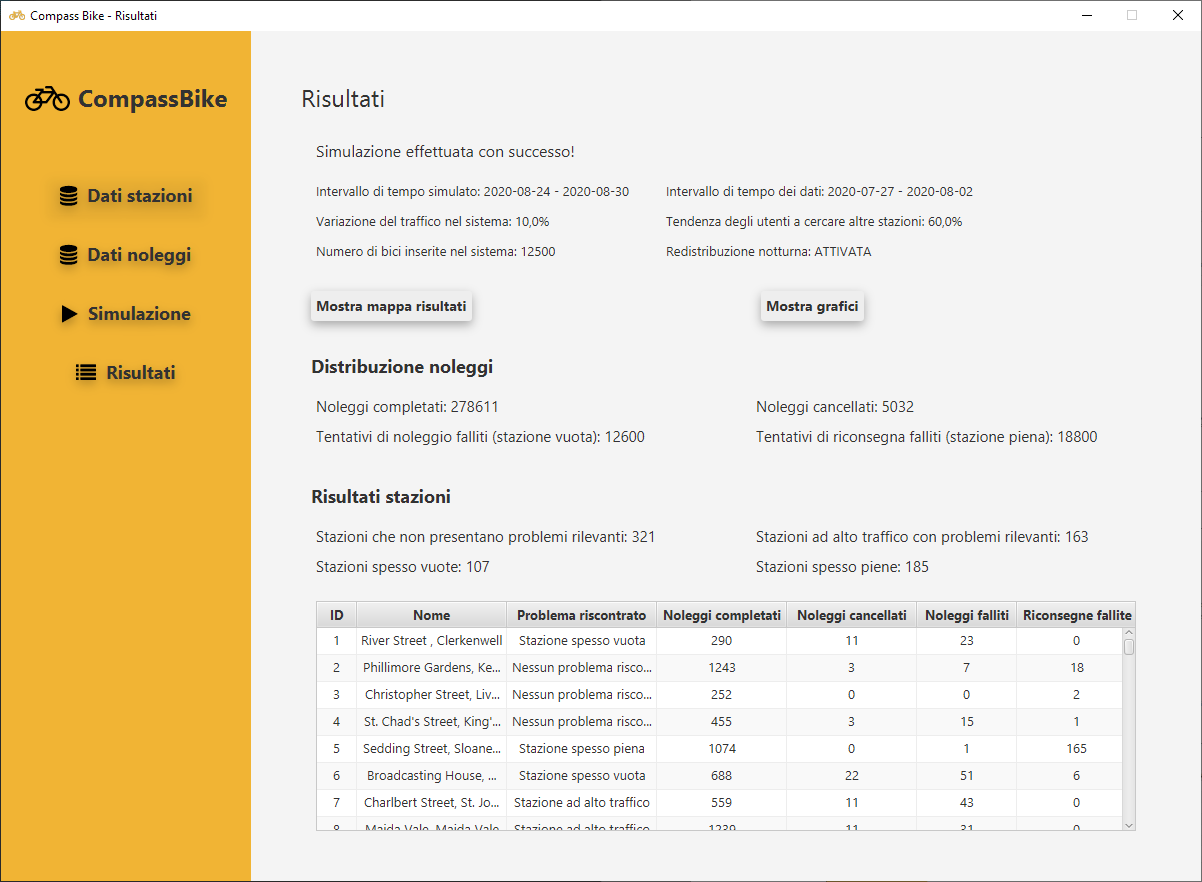
\includegraphics[height=0.47\textheight]{resources/images/screenshot/Result.png} \hspace*{\fill}
	\end{figure}	

	\begin{figure}[H]
	\caption{Schermata grafici}
	\label{charts}
	\hfill 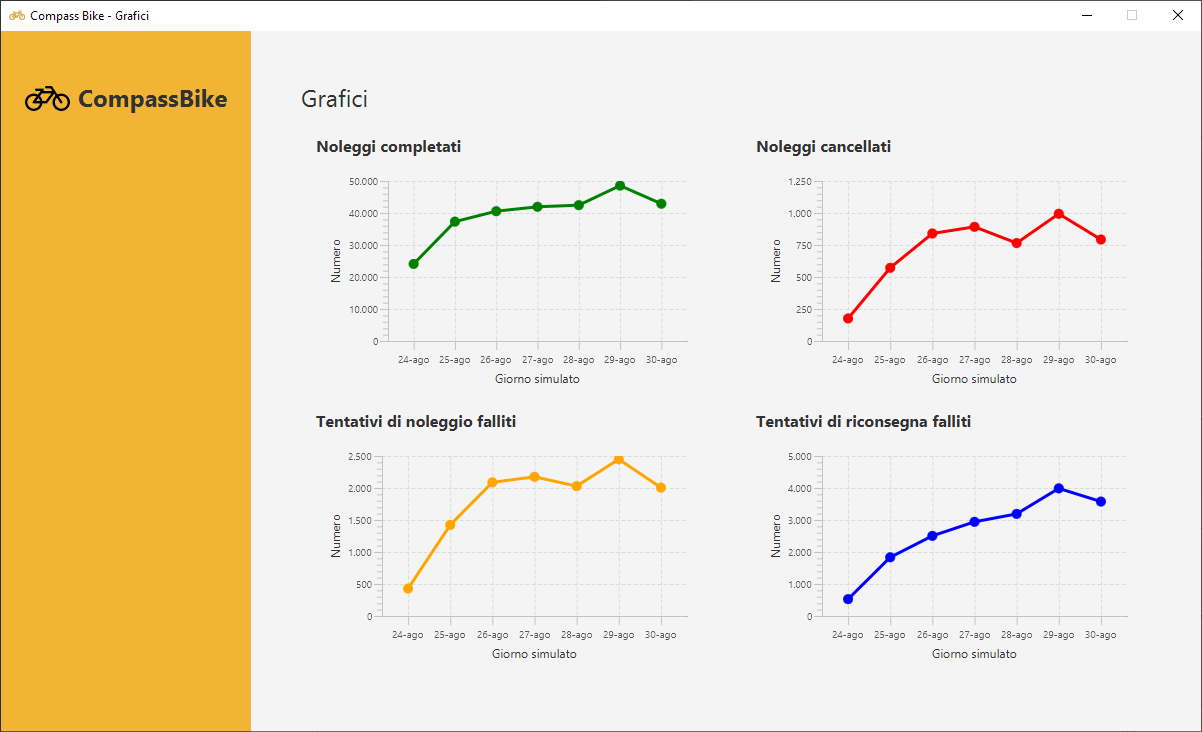
\includegraphics[width=\textwidth]{resources/images/screenshot/Charts.png} \hspace*{\fill}

	\caption{Mappa risultato}
	\label{map}
	\hfill 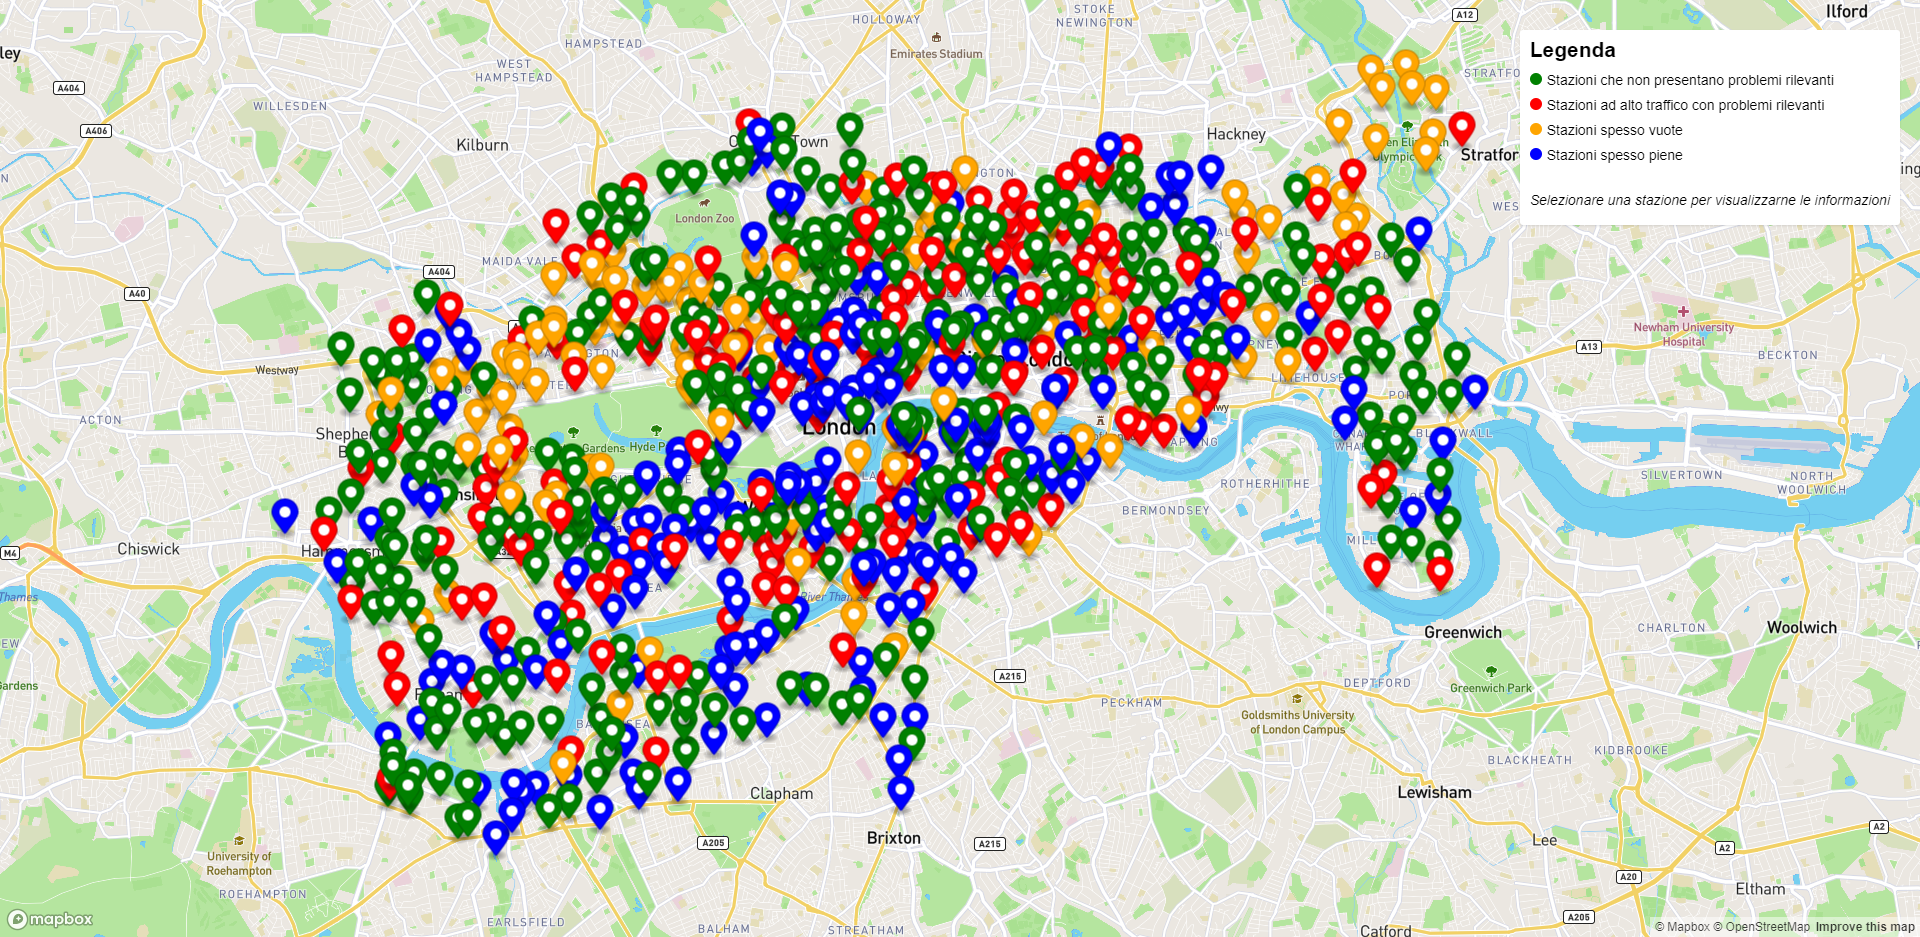
\includegraphics[width=\textwidth]{resources/images/screenshot/Map.png} \hspace*{\fill}
	\end{figure}	
	

\newpage

%__________ESEMPIO E RISULTATI__________

\section{Esempio d'uso e risultati}

	\subsection{Parametri}
	Si riportano i parametri inseriti all'avvio della simulazione utilizzati per gli esempi che seguono.
	\begin{itemize}
	\item Intervallo di tempo da simulare:
		\begin{itemize}
		\item Data di inizio: 24-08-2020
		\item Data di fine: 30-08-2020
		\end{itemize}
	\item Intervallo di tempo dei dati da utilizzare:
		\begin{itemize}
		\item Data di inizio: 27-07-2020
		\item Data di fine: 02-08-2020
		\end{itemize}
	\item Aumento o diminuzione percentuale di traffico: 10.0\%
	\item Tendenza degli utenti a recarsi in un'altra stazione: 60.0\%
	\item Numero di biciclette: 12000
	\end{itemize}

	\begin{figure}[H]
	\caption{Grafici esempio 1}
	\label{charts1}
	\hfill 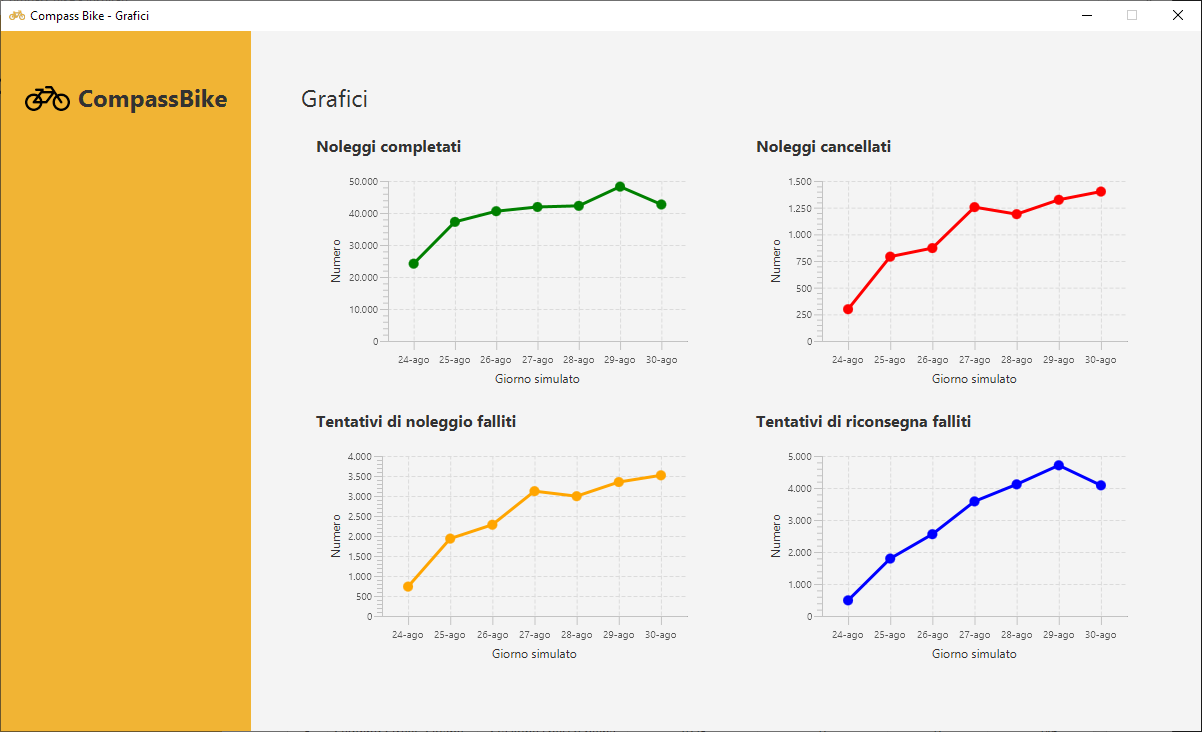
\includegraphics[width=\textwidth]{resources/images/screenshot/ChartsExample1.png} \hspace*{\fill}
	\end{figure}

	\subsection{Analisi}
	La prima simulazione svolta fornirà anche i "valori di controllo" utili ad analizzare le differenze causate dalla modifica dei parametri o del sistema negli esempi successivi.\\\\
Osservando i grafici in figura \ref{charts1} possiamo immediatamente notare alcune informazioni interessanti:
	\begin{itemize}
	\item L'andamento della linea relativa ai noleggi completati è crescente e presenta un picco sabato 29 e domenica 30 agosto. 
	\item Il fatto che l'andamento della linea relativa ai tentativi di noleggio falliti e quella relativa ai noleggi cancellati sia simile è dovuto al fatto che i noleggi cancellati avvengono a seguito di un certo numero di tentativi di noleggio falliti, a causa della mancanza di bici da poter noleggiare nelle stazioni. Inoltre, queste due linee presentano un andamento crescente in quanto i parametri che rappresentano dipendono dal traffico del sistema in un determinato giorno. 
	\item Infine, la linea relativa ai tentativi di riconsegna falliti presenta un andamento crescente molto più netto: una riconsegna fallisce nel caso in cui la stazione scelta dall'utente risulti piena. Questo andamento è molto più interessante dei precedenti in quanto evidenzia come questo parametro sia solo in parte connesso al traffico nel sistema, in altre parole, l'andamento significativamente crescente è dovuto al fatto che il normale utilizzo del servizio da parte degli utenti porta nel lungo periodo ad avere una distribuzione dei mezzi nel sistema non uniforme, portando alla creazione di zone ad alto tasso di biciclette ma in cui il numero di noleggi non è così elevato.\\
Questa conclusione ci viene confermata analizzando la mappa in figura \ref{map1} dove possiamo chiaramente notare due vaste zone che presentano quasi esclusivamente stazioni spesso piene (codificate in blu).\\\\
	\end{itemize}
	\begin{figure}[H]
	\caption{Mappa esempio 1}
	\label{map1}
	\hfill 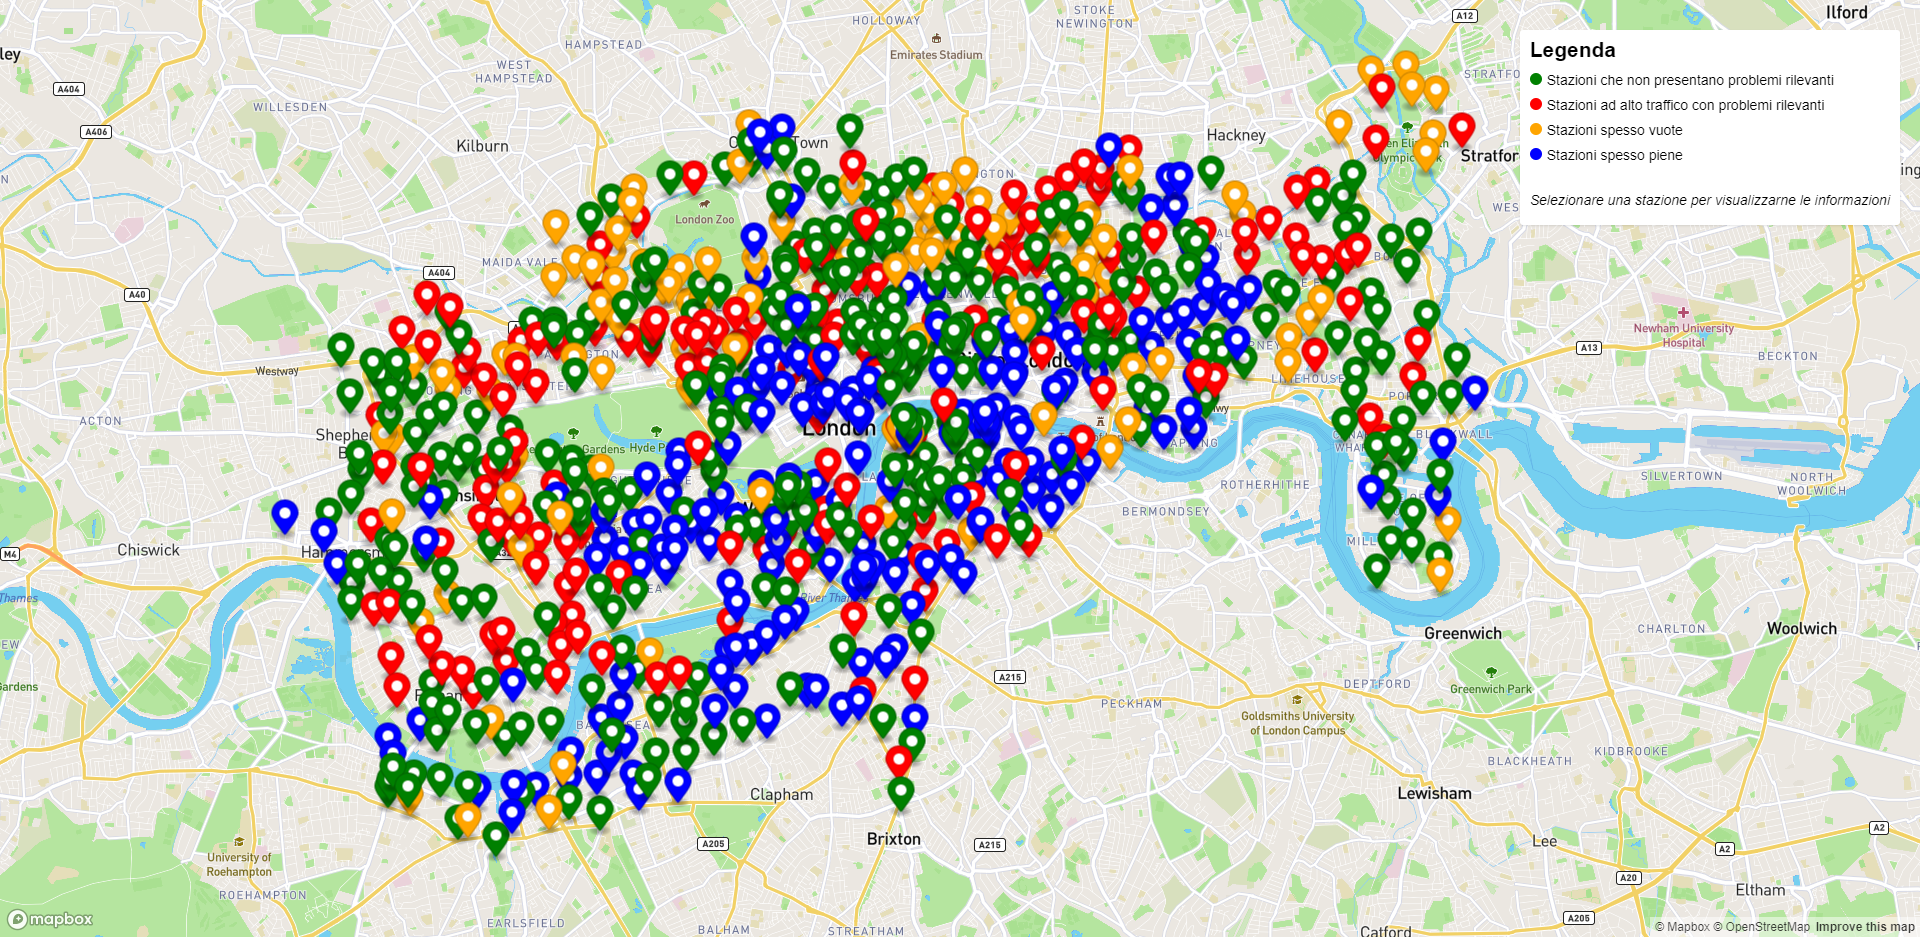
\includegraphics[width=\textwidth]{resources/images/screenshot/MapExample1.png} \hspace*{\fill}
	\end{figure}	
	\begin{figure}[H]
	\caption{Grafici esempio 2}
	\label{charts2}
	\hfill 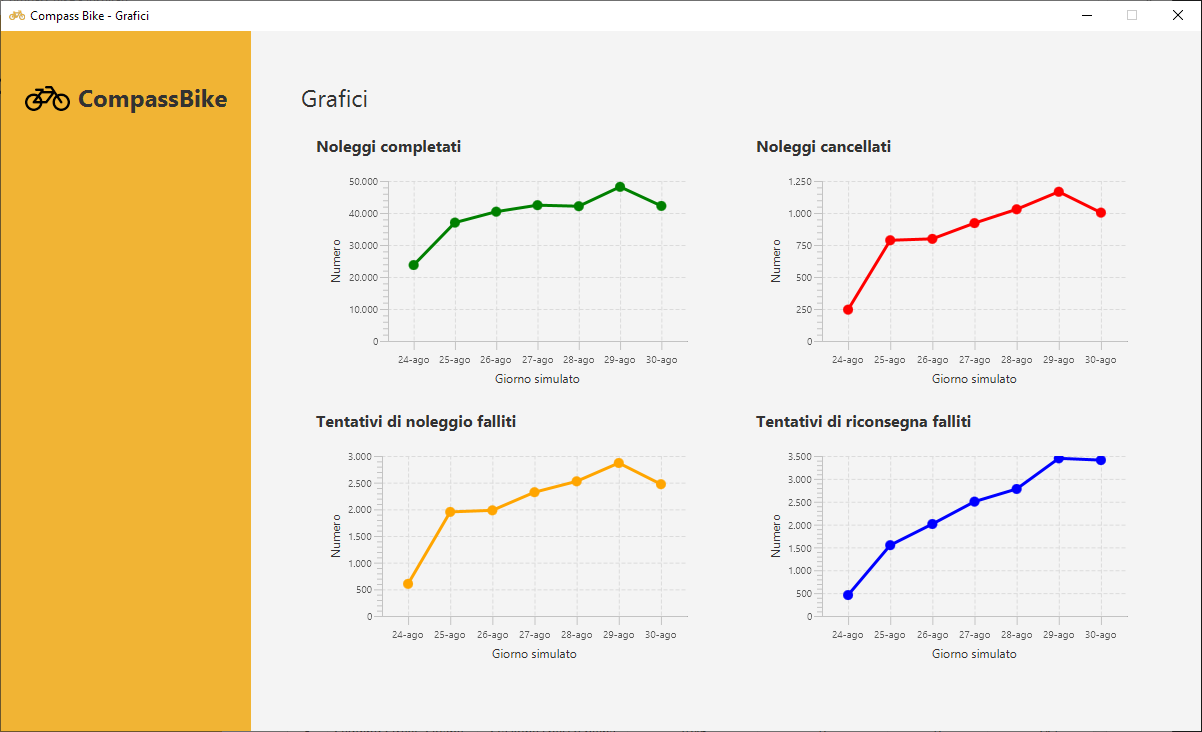
\includegraphics[width=\textwidth]{resources/images/screenshot/ChartsExample2.png} \hspace*{\fill}
	\end{figure}
\newpage

In figura \ref{charts2} possiamo vedere i risultati ottenuti con gli stessi parametri in input, ma attivando la ridistribuzione notturna dei mezzi.\\
Analizzando i grafici, soprattutto quello relativo ai tentativi di noleggio falliti e quello relativo ai tentativi di riconsegna falliti, possiamo vedere prima di tutto come l'entità delle criticità si sia molto ridotta. La linea blu mantiene un andamento crescente, non così netto come il caso precedente, invece, la linea gialla presenta un andamento crescente di minore entità, soprattutto nei giorni centrali del periodo simulato, a dimostrazione di come l'utilizzo di una strategia di ridistribuzione generi un miglior bilanciamento dei mezzi all'interno del sistema.\\
In tabella \ref{tabex1} sono riportati i valori relativi alla simulazione senza ridistribuzione e in tabella \ref{tabex2} quelli ottenuti con l'attivazione della ridistribuzione.\\
	\begin{table}[!htb]
	\begin{minipage}{0.45\linewidth}
	    \centering
	    \caption{Risultati senza\\ ridistribuzione}
	    \label{tabex1}
	\begin{tabular}{| c | c |} 
	 \hline
	 \textbf{Categoria} & \textbf{Numero} \\ [0.5ex] 
	\hline
	 \hline
	 Completati & 277811 \\
	 \hline
	 Cancellati & 7130 \\  
	 \hline
	 Noleggi falliti & 17938 \\
	 \hline
	 Riconsegne fallite & 21581 \\
	 \hline
	\end{tabular}
	\end{minipage}\hfill
	\begin{minipage}{0.45\linewidth}
	    \centering
	    \caption{Risultati con\\ ridistribuzione}
	    \label{tabex2}
	\begin{tabular}{| c | c |} 
	 \hline
	 \textbf{Categoria} & \textbf{Numero} \\ [0.5ex] 
	\hline
	 \hline
	 Completati & 276919 \\
	 \hline
	 Cancellati & 5950 \\  
	 \hline
	 Noleggi falliti & 14725 \\
	 \hline
	 Riconsegne fallite & 16367 \\
	 \hline
	\end{tabular}
	\end{minipage}
	\end{table}\\

	\begin{figure}[!b]
	\centering
	\caption{Zona di mappa esempio 3}
	 \begin{subfigure}[b]{0.45\textwidth}
	\centering
	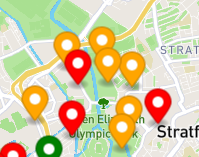
\includegraphics[width=\textwidth]{resources/images/screenshot/MapExample2.png}
    	\caption{Stato iniziale}	
    	\label{submap1}
 	\end{subfigure}\hfill
 	 \begin{subfigure}[b]{0.45\textwidth}
	\centering
    	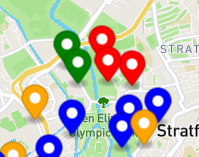
\includegraphics[width=\textwidth]{resources/images/screenshot/MapExample3.png}
    	\caption{A seguito dell'aggiunta}
    	\label{submap2}
  	\end{subfigure}
	\end{figure}

Per mostrare le funzionalità di test delle modifiche apportate al sistema ci si concentrerà sulla zona visibile in figura \ref{submap1} estratta dalla mappa in figura \ref{map1}, notiamo subito che la zona risulta molto critica probabilmente a causa del vicino parco che genera un elevato traffico.\\\\
Possiamo vedere in figura \ref{submap2} come cambi la situazione inserendo una nuova stazione nell'area, oltre che un miglioramento a livello generale, andando a osservare i valori, prima e dopo l'aggiunta, riportati rispettivamente in tabella \ref{tabex3} e \ref{tabex4}, relativi alle singole stazioni della zona si può vedere come si è ottenuta una consistente riduzione dell'entità dei problemi presenti.\\
Parametri stazione inserita:
	\begin{itemize}
		\item Latidutine: 51.539038
		\item Longitudine: -0.007594
		\item Numero docks: 30
	\end{itemize}

	\begin{table}[!htb]
	\begin{minipage}{0.45\linewidth}
	    \centering
	    \caption{Risultati iniziali}
	    \label{tabex3}
	\begin{tabular}{| c | c |} 
	 \hline
	 \textbf{ID stazione} & \textbf{Noleggi falliti} \\ [0.5ex] 
	\hline
	 \hline
	 692 & 83 \\
	 \hline
	 783 & 66\\
	\hline
	784 & 109 \\
	 \hline
	785 & 365 \\
	 \hline
	786 & 101 \\
	 \hline
	787 & 48 \\
	 \hline
	789 & 165 \\
	 \hline
	790 & 76 \\
	 \hline
	812 & 82 \\  
	 \hline
	  816 & 32\\
	 \hline
	 \text{Totale} & 1127\\
	 \hline
	\end{tabular}
	\end{minipage}\hfill
	\begin{minipage}{0.45\linewidth}
	    \centering
	    \caption{Risultati a seguito\\ dell'aggiunta delle stazioni}
	    \label{tabex4}
	\begin{tabular}{| c | c |} 
	 \hline
	 \textbf{ID stazione} & \textbf{Noleggi falliti} \\ [0.5ex] 
	\hline
	 \hline
	 692 & 73 \\
	 \hline
	 783 & 0\\
	\hline
	784 & 23 \\
	 \hline
	785 & 21 \\
	 \hline
	786 & 37 \\
	 \hline
	787 & 30 \\
	 \hline
	789 & 6 \\
	 \hline
	790 & 0 \\
	 \hline
	812 & 0 \\  
	 \hline
	  816 & 0 \\
	 \hline
	Aggiunta & 79 \\
	 \hline
	\text{Totale} & 269 (348)\\
	 \hline
	\end{tabular}
	\end{minipage}
	\end{table}


\newpage

%__________CONCLUSIONI__________

\section{Conclusioni e possibili miglioramenti}

In conclusione, l'applicazione sviluppata raggiunge gli obiettivi posti in fase di progettazione seppur con alcune limitazioni già indicate al paragrafo \ref{crit}.\\
Permette sia di ottenere una visione generale sullo stato del sistema, ma anche di analizzare il rendimento della singola stazione.\\
Inoltre, come mostrato negli esempi, permette, in maniera semplice, di analizzare le conseguenze delle possibili modifiche attuabili sul sistema.\\\\
Uno sviluppo interessante potrebbe essere l'aggiunta di indicatori economici che si basino, per esempio, sul listino prezzi del servizio in esame e su eventuali minuti gratuiti concessi agli utenti. Tali indicatori potrebbero essere usati per valutare la perdita economica derivante dai problemi che il sistema presenta e, di conseguenza, per valutare il ritorno economico dovuto a un eventuale risoluzione degli stessi, in modo da permettere la valutazione del vantaggio economico derivato dagli interventi necessari a risolvere tali criticità.\\\\
Inoltre, come già detto, potrebbe essere introdotta una funzione che possa gestire il danneggiamento dei mezzi e i conseguenti interventi di riparazione.\\\\\\
Infine, soffermandosi ad analizzare i tempi di esecuzione dell'applicazione, si possono trarre le seguenti conclusioni:\\
	\begin{itemize}
	\item Per quanto riguarda l'algoritmo di simulazione, il tempo di esecuzione richiesto risulta soddisfacente, considerando il numero di eventi che vengono processati: in media 800000 eventi per un periodo di simulazione pari a una settimana. Questo numero si traduce in circa 12 secondi di esecuzione, tempo che diminuisce drasticamente con la riduzione dell'ampiezza dell'intervallo di simulazione, arrivando a meno di 300ms nelle simulazioni di un singolo giorno.
	\item Dall'altro lato, invece, l'algoritmo di generazione eventi è meno soggetto a variazioni del tempo di esecuzione dovuto dall'ampiezza dell'intervallo simulato. In questo caso, è richiesto un tempo medio di 11 secondi per la simulazione di una settimane che si riduce, in maniera non molto consistente, a differenza del caso precedente, a circa 4 secondi nelle simulazioni di un singolo giorno. Ciò è dovuto al fatto che questo algoritmo si occupa di effettuare una serie di letture di informazioni aggregate dal database necessarie a inizializzare le strutture dati, infatti, circa il 60\% dei tempi precedentemente indicati è richiesto per effettuare queste letture.
	\end{itemize}
Tenendo conto di queste considerazioni, si ritiene che il margine di miglioramento dei tempi di esecuzione dell'applicazione sia nella possibilità di elaborare query SQL più ottimizzate per estrarre le informazioni dal database.

\newpage

%__________LICENZA__________

\vspace*{\fill}
\begin{center}
\doclicenseImage\\
\doclicenseLongText 
\end{center}

\end{document}
